% Ideia desse capitulo: Apresentar o desenvolvimento do projeto-

%% Revisado por Gabriel Saraiva
%% Revisado por Renata

% Restrições do projeto atual         OK
% Propostas de melhorias                OK
% Documentação do Projeto               OK
% Adaptação do servidor python          OK
% Implementação do cliente Android      OK

\chapter{Descrição e desenvolvimento do projeto}
\label{cap3}

    Neste capítulo são apresentados o desenvolvimento da proposta do projeto e também sua implementação no FlexA. Inicialmente serão abordados as restrições encontradas no projeto atual e a motivação para corrigi-las. Então será apresentada a documentação desenvolvida para que o projeto possa ser viável a longo prazo, então serão detalhadas as adaptações realizadas no módulo servidor para que esse passe a ser compatível com a nova especificação. Por fim, com o novo servidor pronto, será apresentada a implementação do cliente para Android.
    
    %% Para não avacalhar com o projeto do Mario (rsrsrs eu ri disso)... O termo é muito engraçado. Não fiz por mal =)
    
    \section{Restrições da versão atual do FlexA}
    
        A versão atual do FlexA, ainda em um estágio inicial de desenvolvimento, carece de um modelo de programação bem definido, sua documentação precisa ser aprofundada e não menos importante de um protocolo de comunicação precisa ser bem explicitado.
        
        Os principais pontos abordados nesse projeto são:
        
        \begin{itemize}
            \item Documentação inicial do projeto, como um diagrama de classes, casos de uso e também um diagrama com os módulos do sistema e como eles se integram.
            \item Formalização do protocolo de comunicação.
            \item Adaptação incremental do módulo servidor para que ele passe a ser compatível com a documentação gerada.
            \item Implementação do módulo cliente para Android.
        \end{itemize}
        
        A motivação para essas melhorias é que elas fornecerão uma base sólida para que no futuro possam ser incorporados no projeto atual os resultados de trabalhos já realizados em versões anteriores do FlexA, que são listados pelos títulos:
        
        \begin{itemize}
            \item Detecção de Falhas de Comunicação e Balanceamento de Carga no FlexA ~\cite{danilo};
            \item Metodologia para Recuperação de Falhas e Garantia de Disponibilidade no FlexA ~\cite{thiago};
            \item Implementação e avaliação de desempenho de algoritmo de criptografia em GPU para o FlexA ~\cite{leandro};
            \item Sincronização, consistência e falhas no FlexA ~\cite{matheus};
            \item Disponibilidade em um sistema de arquivos distribuído flexível e adaptável ~\cite{lucio};
        \end{itemize}
        
       
    Além de tornar mais fácil a incorporação dos resultados obtidos com os trabalhos citados, a nova documentação deve tornar o sistema fácil de se manter e evoluir e permitir que diversas equipes colaborem com o trabalho de forma simultânea.
    
    
        
    \section{Documentação do projeto}
        
    Um estudo a fundo do sistema foi feito, utilizando a documentação que existia e a análise do código-fonte, para entender o funcionamento e comportamento do sistema e também como era definida a estrutura atual do projeto. 
    
    \subsection{Módulos do Sistema}
    
        Para representar o sistema de forma mais abstrata foi criado um diagrama dos módulos do sistema atual, e suas dependências conforme pode ser visto na Figura \ref{fig:pacotesMario}.
        
        \begin{figure}[!ht]
            \centering
            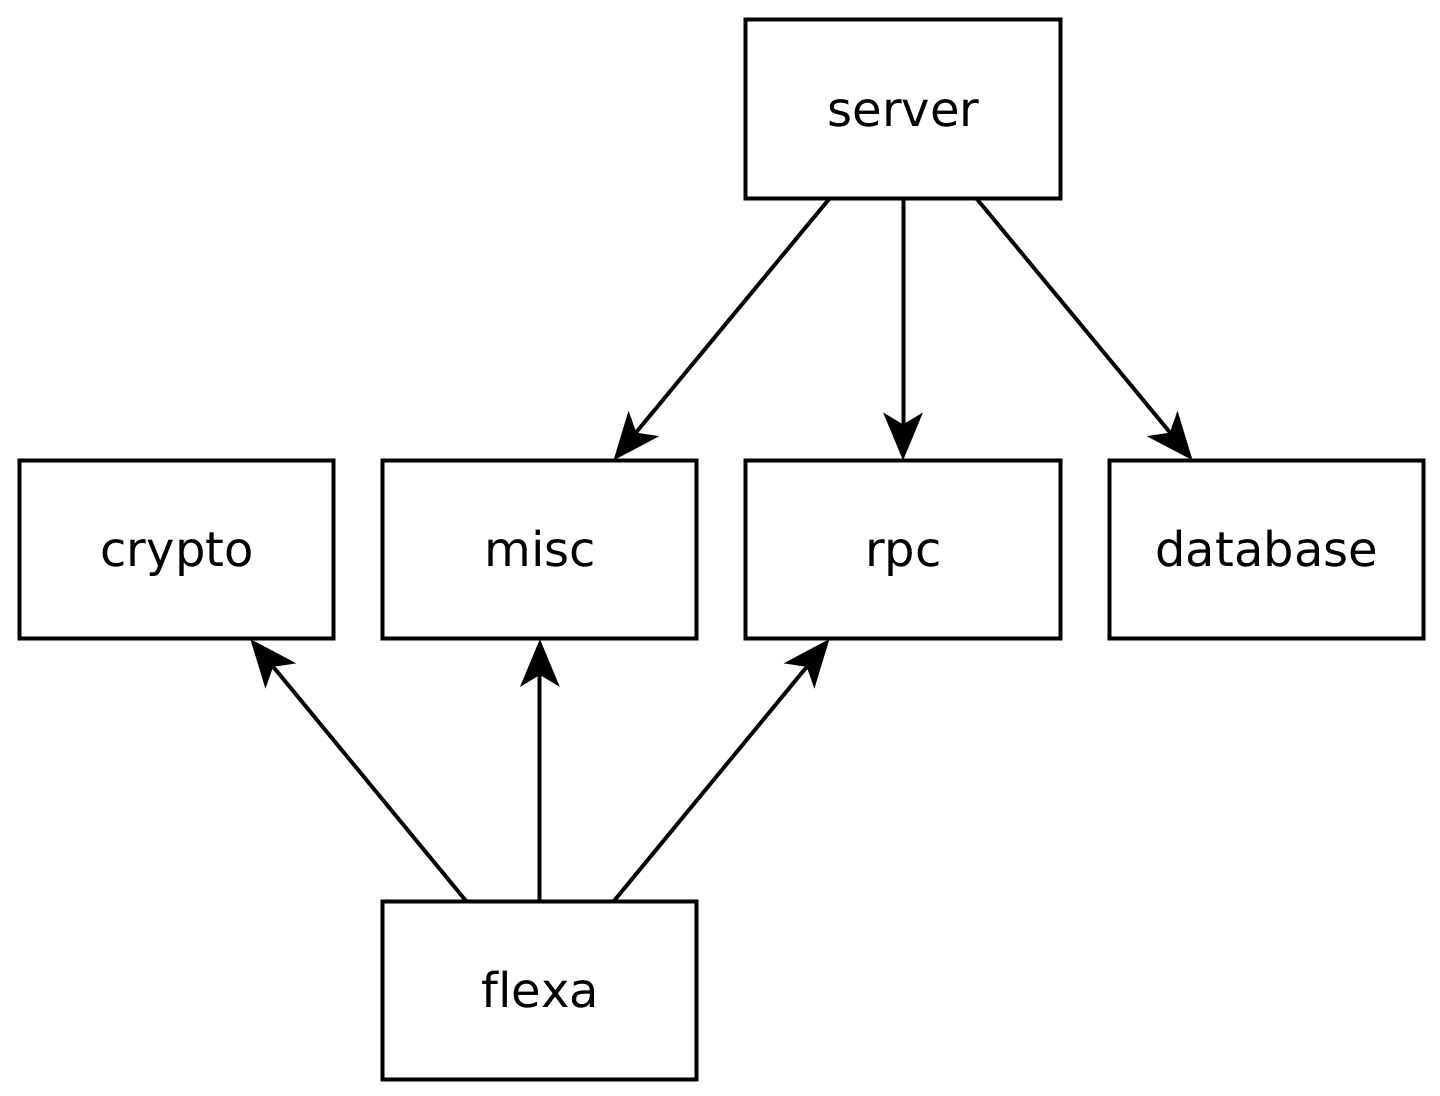
\includegraphics[width=10cm]{pacotesMario.png}
            \caption{Módulos do sistema atual e suas dependências. Criado com base no código fonte do projeto de ~\citeonline{mario}.}
            \label{fig:pacotesMario}
        \end{figure}
        
        Esse diagrama foi gerado a partir do estudo do código-fonte da versão atual do projeto. Apenas por esse diagrama já é possível notar que o módulo Servidor não utiliza os serviços de criptografia, e que apenas o servidor tem acesso aos bancos de dados de metadados, o que ajuda a evidenciar a segurança dos dados do cliente que já chegam aos servidores criptografados.
    
    \subsection{Diagrama de classes do sistema existente} 
    
        Para que fosse possível analisar a estrutura mais interna dos módulos foi criado o diagrama de classes da \textit{Unified Language Model} (UML)~\cite{umlClasses}. Esse diagrama é apresentado na figura \ref{fig:classesMario}. Embora seja um diagrama de classes, alguns abusos de notação tiveram que ser utilizados devido a lacuna existente entre a representação dos diagramas de classes e a linguagem Python em que o FlexA é desenvolvido. Esses abusos são a representação do código que não pertence a nenhuma classe, mas estão dentro de módulos, e também o uso de pacotes para representar arquivos.
        
        \begin{figure}[!ht]
        \centering
        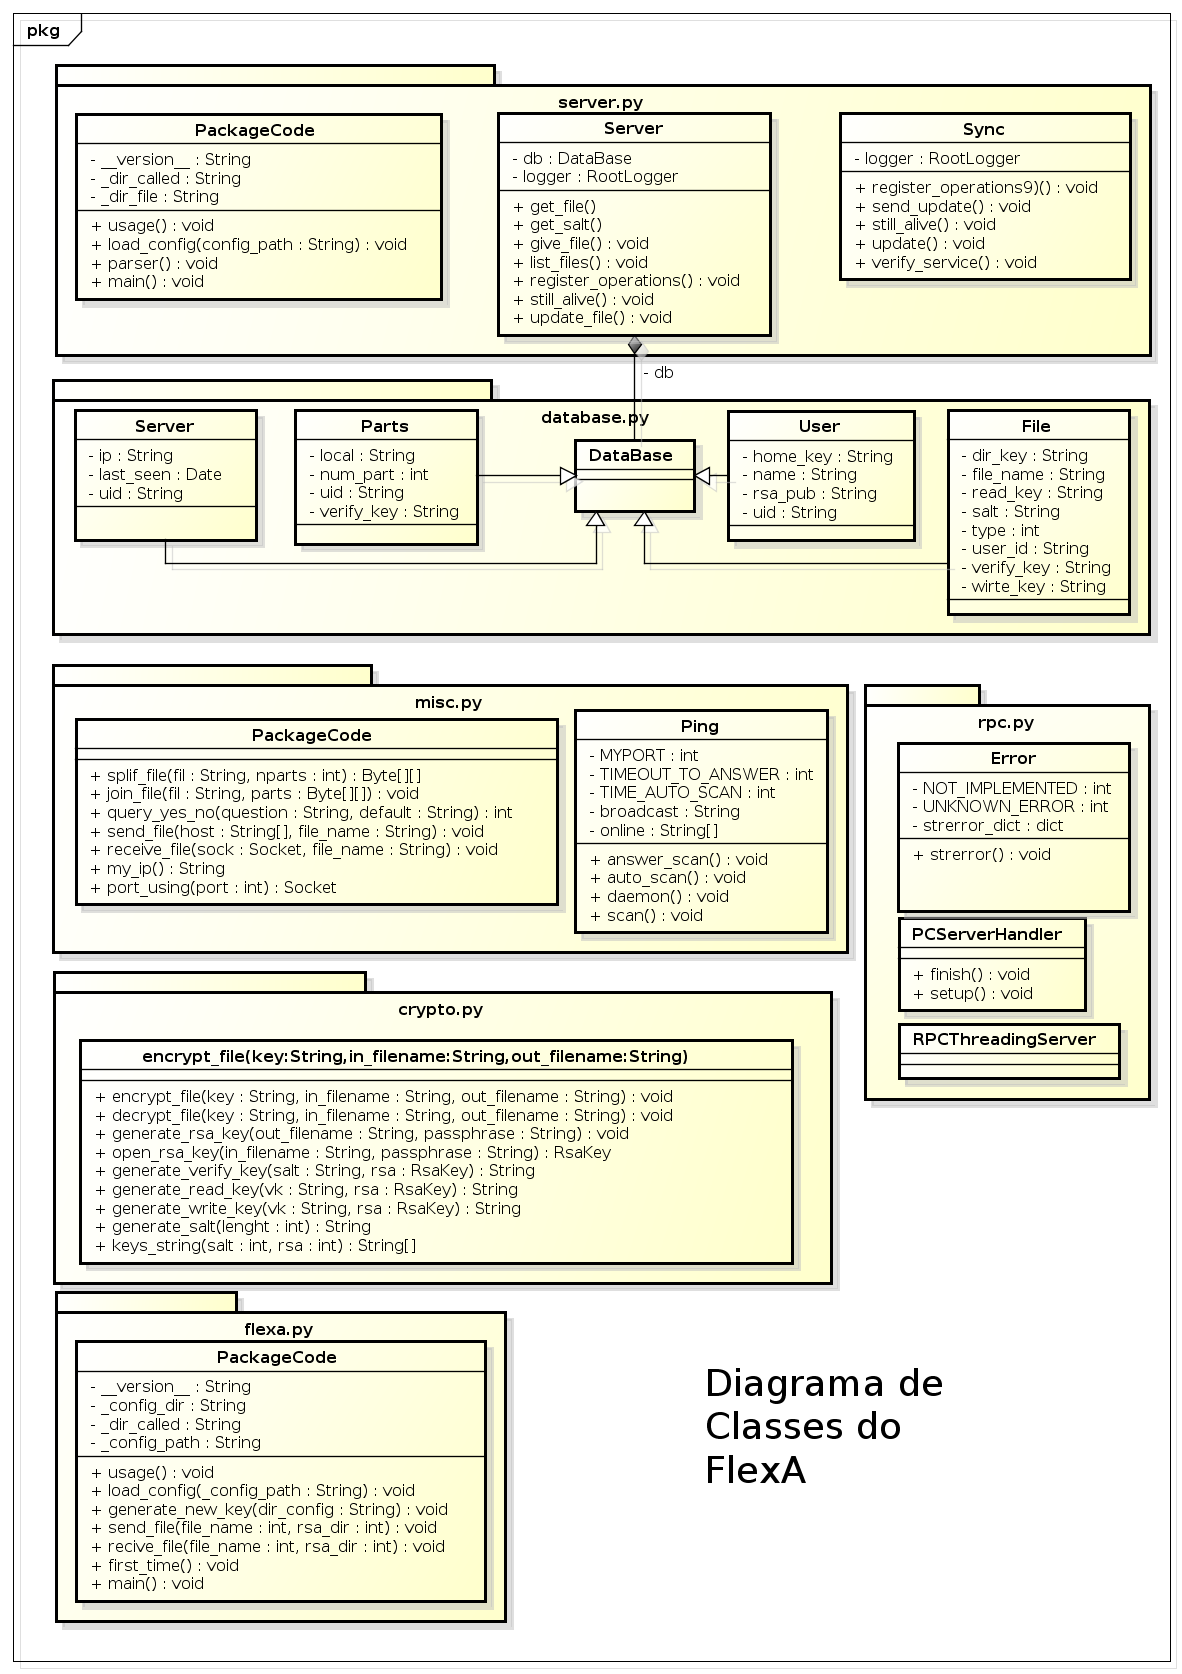
\includegraphics[width=12cm]{classesMario.png}
        \caption{Classes e pacotes (arquivos) que estruturam a versão atual do FlexA}
        \label{fig:classesMario}
        \end{figure}
             
        
        Para que o FlexA seja mais aberto e flexível é necessário realizar adaptações no código afim de fazer uma melhor separação das funções e dos módulos.
        
        \subsection{Diagrama de Casos de Uso}
        
        Para que fosse possivel elaborar a adaptação do projeto, num primeiro momento foi feito o levantamento dos requisitos do FlexA, junto com os objetivos de melhoria do código existente. Dessa forma foi elaborado um diagrama UML de casos de uso de acordo com ~\cite{umlCasosDeUso}. O diagrama com os casos de uso é apresentado na Figura \ref{fig:casosDeUsoGabriel}.
        
        \begin{figure}[!ht]
        \centering
        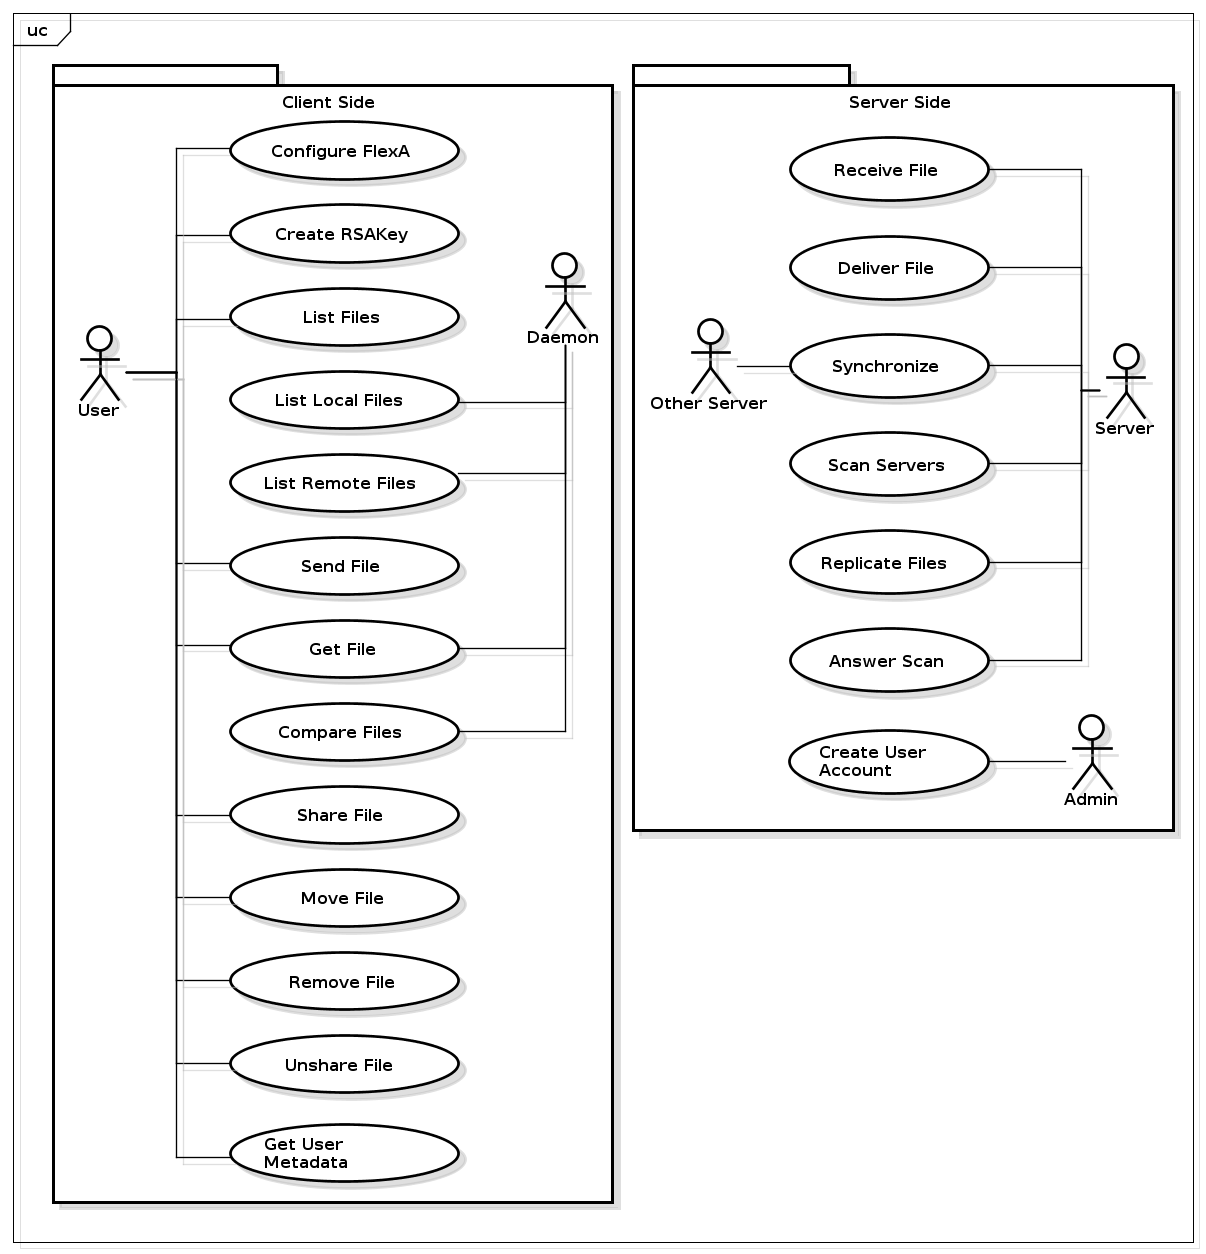
\includegraphics[width=12cm]{casosDeUsoGabriel.png}
        \caption{Diagrama de Casos de uso com os requisitos funcionais do FlexA.}
        \label{fig:casosDeUsoGabriel}
        \end{figure}
    
        Dos casos de uso apresentados na figura \ref{fig:casosDeUsoGabriel}, serão implementados e utilizados nesse trabalho apenas os referentes ao módulo cliente devido ao escopo do projeto. Os restantes foram definidos juntos para preparar os trabalhos futuros.
        
        \subsection{Interface de Comunicação Cliente-Servidor}
        
        Já com os objetivos do trabalho definidos, e uma documentação do que existia que permitisse entender o projeto, foi então formulada a interface que servirá de alicerce desse trabalho que será responsável por padronizar e fornecer as comunicações entre o cliente e o servidor. Essa interface, que é apresentada na figura   \ref{fig:interfaceComunicacao}, foi desenvolvida em reunião com os outros desenvolvedores do FlexA para que fossem atendidas todas as necessidades do trabalho atual e também do FlexA como um todo no futuro.
       
        \begin{figure}
        \centering
        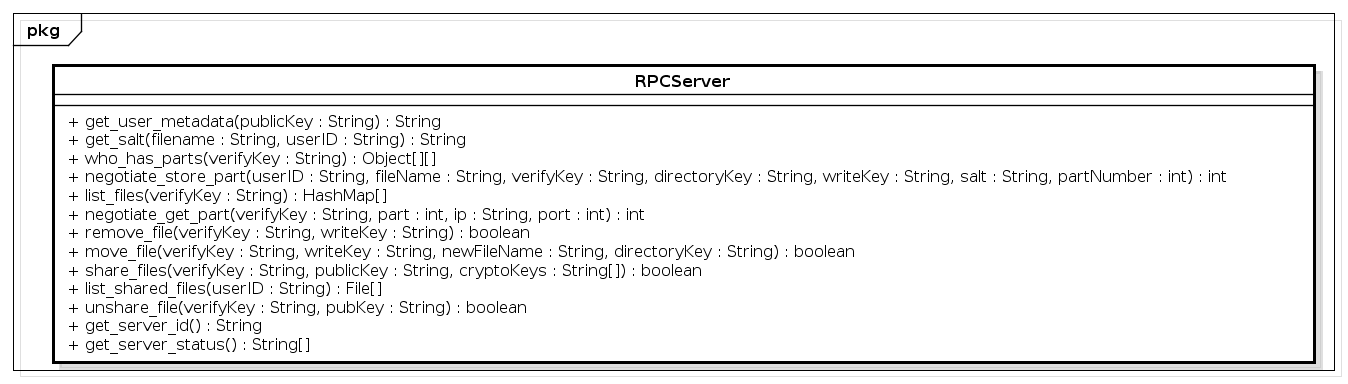
\includegraphics[width=15cm]{interfaceCom.png}
        \caption{Interface de comunicação dos servidores do FlexA.}
        \label{fig:interfaceComunicacao}
        \end{figure}
        
        Essa interface é de grande importância para o projeto, pois é ela que servirá como referência para o desenvolvimento do módulo cliente e também do módulo servidor, uma vez que define os métodos que deverão ser invocados durante a comunicação entre os clientes e os servidores, utilizando XML-RPC e independendo da linguagem utilizada.
        
        \subsection{Protocolos de Comunicação Cliente-Servidor}
        
        Com as funcionalidades que são esperadas do sistema e a interface de comunicação definida, foi feita a análise das comunicações entre cliente e servidor. Formalizou-se então os protocolos de comunicação, utilizando a notação para protocolos de comunicação apresentada em ~\cite{ross} que é mostrada na tabela \ref{tab:notacao}. 
        
        \begin{table}[!ht]
        
        \centering
        \begin{tabular}{|l|l|}
        \hline
        
        $C$ & módulo cliente \\
        \hline
        $S$ & módulo servidor \\
        \hline
        $privKey_{X}$ & chave privada $X$ \\
        \hline
        $pubKey_{X}$ & chave pública $X$ correspondente a $privKey_{X}$\\
        \hline
        $C \rightarrow S : dado$ & $C$ envia $dado$ para $S$\\
        \hline
        $C \rightarrow S : {dado}_{pubKey_{x}}$ & $C$ envia $dado$ criptografado com a chave pública $X$ para $S$\\
        \hline

        \end{tabular}
        \caption{Notação utilizada para definição de protocolos de comunicação ~\cite{ross}.}
        \label{tab:notacao}
        \end{table}
        
        Formalizadas as definições que serão utilizadas a seguir, são apresentados os protocolos para as comunicações. Esses protocolos foram elaborados com base no código fonte ~\cite{mario} e na interface de comunicação apresentada, já inserindo as adaptações para fornecer maior modularização, compatibilidade e segurança ao sistema.
        
        \subsubsection{Protocolos de manipulação de arquivos}
        
        A primeira formalização é o protocolo para solicitação dos metadados do usuário, que é feita quando o FlexA é iniciado pela primeira vez ou caso seja necessário obter o \textit{userID} do usuário. Isso é feito com base em sua chave pública previamente cadastrada no sistema por um administrador. O protocolo é apresentado na figura \ref{fig:protMetadadosUsuario}. Esse protocolo é implementado pela função \textit{get\_user\_metadata}, que é apresentada na figura \ref{fig:interfaceComunicacao}.
        
        \begin{figure}[!ht]
        
        \bordaProtocolo{
                $C \rightarrow S: pubKey_{C}$ \\
                $S \rightarrow C: \{userID,homeKey\}_{pubKey_{C}}$
        }
        
        \caption{Protocolo de requisição dos metadados de um usuário com base na sua chave pública.}
        \label{fig:protMetadadosUsuario}
        \end{figure}
        
        Com os metadados do usuário (\textit{userID} e \textit{homeKey} que é o identificador de sua pasta raiz) o usuário pode começar a utilizar o sistema enviando e recebendo arquivos.
        
        Para que o usuário possa enviar um arquivo para o sistema é necessário verificar se existe um arquivo com o mesmo nome no mesmo endereço especificado através do \textit{salt}. Caso o arquivo não exista ainda, é feito o cadastro e solicitado o \textit{salt} referente ao arquivo. Na figura \ref{fig:protGetSalt} é formalizado o protocolo de requisição do \textit{salt} de um arquivo. É importante ressaltar que \textit{fileName} é composto pelo nome completo do arquivo com o diretório em que o arquivo se encontra. Esse endereço é relativo ao diretório mapeado do FlexA para o usuário. Esse protocolo é implementado pela função \textit{get\_salt}, que é apresentada na figura \ref{fig:interfaceComunicacao}.

        \begin{figure}[!ht]
        \bordaProtocolo{
            $C \rightarrow S: fileName,userID$ \\
            $S \rightarrow C: salt$
        }
        \caption{Requisição do \textit{salt} de um arquivo.}
        \label{fig:protGetSalt}
        \end{figure}
        
        Caso o \textit{salt} retornado pelo servidor seja igual $0$ é assumido que esse arquivo ainda não existe no servidor, e então o próprio cliente gera um \textit{salt} para esse arquivo.
        
        Já com o \textit{salt}, o módulo cliente gera o trio de chaves para o arquivo (VK, RK e WK) de acordo com a figura \ref{fig:chavesFlexa} , criptografa o arquivo utilizando a RK, faz a divisão do arquivo em $N$ porções de acordo com o tamanho do arquivo, ($N$ e o tamanho do arquivo são configurações definidas pelo usuário) caso necessário e envia cada porção para um servidor. Primeiro o módulo cliente faz o cadastro do arquivo no servidor e então envia as porções. Na figura \ref{fig:protSendFile} é descrito o protocolo utilizado no cadastro do arquivo, onde $N$ é o número de porções em que o arquivo foi dividido, $directoryKey$ é o identificador do diretório que o arquivo está e $fileType$ é o tipo do arquivo (diretório ou arquivo comum). Esse protocolo é implementado pela função \textit{negociate\_store\_part}, que é apresentada na figura \ref{fig:interfaceComunicacao}.
        
        \begin{figure}[!ht]
        \bordaProtocolo{
            Para $i$ de $1$ até $N$: \\
            $C \rightarrow S_{i}: userID,fileName,verifyKey,directoryKey,writeKey,salt,partNumber_{i}$ \\
            $S_{i} \rightarrow C: port $
        }
        
        \caption{Cadastro do arquivo nos servidores e negociação da porta de envio do arquivo}
        \label{fig:protSendFile}
        \end{figure}
        
        Após o cadastro do arquivo e a negociação da porta de transmissão do arquivo, é feita a transmissão do arquivo em uma nova conexão com o servidor na porta $port$.
        
        Com a negociação pronta basta enviar para o servidor a porção correspondente. Essa comunicação é definida conforme o protocolo mostrado na figura \ref{fig:protSendFileData}. Esse protocolo é implementado através de \emph{sockets}, sem o uso do XML-RPC, por questões de desempenho.
        
        \begin{figure}[!ht]
        \bordaProtocolo{
            Para $i$ de $1$ até $N$: \\
            $C \rightarrow S_{i}: filePart_{i}$
        }
        \caption{Transmissão das porções dos arquivos aos servidores, feito via socket.}
        \label{fig:protSendFileData}
        \end{figure}
        
        
        Com os protocolos já definidos é possível enviar um arquivo para o servidor. Mas ainda não é possível recuperá-lo. A seguir serão tratados os protocolos envolvidos na recuperação dos arquivos enviados aos servidores.
        
        Para recuperar um arquivo, é de grande importância a capacidade de listar os arquivos de um diretório. Para essa ação é utilizado o protocolo da figura \ref{fig:protListFiles}. Esse protocolo é implementado pela função \textit{list\_files}, que é apresentada na figura \ref{fig:interfaceComunicacao}.
        
        \begin{figure}[!ht]
        \bordaProtocolo{
            $C \rightarrow S: directoryKey$\\
            $S \rightarrow C: metaFile_{0}, metaFile_{1}, metaFile_{2},...,metaFile_{n}$
        }
        \caption{Requisição da lista dos arquivos em um diretório}
        \label{fig:protListFiles}
        \end{figure}
        
        Ao requisitar ao servidor os arquivos do diretório referenciado por $directoryKey$, o servidor manda pacotes de informação $metaFile$ referente aos arquivos. Cada pacote desse é composto por:
        \begin{itemize}
            \item nome do arquivo
            \item tamanho do arquivo
            \item dono do arquivo
            \item data de criação
            \item data de modificação
        \end{itemize}
        
        Essas características do arquivo são enviadas junto com o nome do arquivo para evitar acessos desnecessários ao servidor para recuperar cada uma dessas informações posteriormente. Isso influencia no tempo de resposta do sistema.
        
        Com a lista dos arquivos, o usuário pode requisitar um arquivo específico ao servidor. Ao requisitar o arquivo, o módulo cliente faz a solicitação do \textit{salt} referente ao arquivo pelo atributo nome, com essa informação gera o trio de chaves do arquivo. Com o identificador do arquivo (\textit{verify key}), o cliente solicita a um servidor uma lista com quais servidores possuem as porções do arquivo. Essa comunicação é formalizada na figura \ref{fig:protWhoHasParts}. Esse protocolo é implementado pela função \textit{who\_has\_parts}, que é apresentada na figura \ref{fig:interfaceComunicacao}.
        
         \begin{figure}[!ht]
        \bordaProtocolo{
            $C \rightarrow S: VK, userID$ \\
            $S \rightarrow C: (S_{0},1),(S_{0},2),(S_{1},1),(S_{1},3),(S_{2},2),(S_{2},3),...$
        }

        \caption{Já com a \textit{verify key}, é solicitado uma lista dos servidores que possuem as partes do arquivo}
        \label{fig:protWhoHasParts}
        \end{figure}
        
        Ao fazer a solicitação de quais servidores possuem as partes do arquivo desejado, o cliente recebe uma lista de registros de quais servidores possuem qual parte do arquivo, no seguinte formato: ($SERVIDOR$,$PARTE DO ARQUIVO$). Esse é o formato utilizado na figura \ref{fig:protWhoHasParts}.
        
        Com a lista dos servidores que possuem as partes do seu arquivo o cliente pode finalmente requisitar as partes do arquivo. Esse processo é feito de acordo com o protocolo apresentado pela figura \ref{fig:protNegociateGetPart} e é implementado pela função \textit{negociate\_get\_parts}, que é apresentada na figura \ref{fig:interfaceComunicacao}.
        
        \begin{figure}[!ht]
        \bordaProtocolo{
            Para $i$ de $1$ até $N$:\\
                $C \rightarrow S_{i}: verifyKey,part{i},ip,port$
        }
        \caption{Módulo cliente envia informação para os servidores, negociando o recebimento das partes}
        \label{fig:protNegociateGetPart}
        \end{figure}
        
        Esse protocolo diz que o cliente é quem irá abrir a conexão para receber o arquivo, e o servidor ira se conectar com o cliente utilizando o $ip$ e $port$ para isso. Após conectado com o cliente o servidor enviará o arquivo para o cliente baseado pelo protocolo apresentado pela figura\ref{fig:protGetPart}. Uma vez que esse protocolo também não é feito via XML-RPC não é definida uma função específica.
        
        \begin{figure}[!ht]
        \bordaProtocolo{
            Para $i$ de $1$ até $N$:\\
                $S_{i} \rightarrow C: filePart_{i}$
        }
        \caption{Servidores enviando porções do arquivo para o cliente}
        \label{fig:protGetPart}
        \end{figure}
        
        
        
        Uma vez que o cliente tenha todas as partes do arquivo a junção dessas partes é feita e o arquivo é descriptografado utilizando a chave de criptografia \textit{read key} que apenas o cliente possui.
        
        A operação de atualização de um arquivo nos servidores é equivalente a remover o arquivo atual e cadastrar um novo arquivo. Como o protocolo de envio de arquivos já foi apresentado nas figuras \ref{fig:protSendFile} e \ref{fig:protSendFileData}, são feitas a seguir a definição do protocolo de remoção de um arquivo dos servidores. Esse protocolo é apresentado na figura \ref{fig:protRemoveFile} e é implementado pela função \textit{remove\_file} da figura \ref{fig:interfaceComunicacao}.
        
        \begin{figure}[!ht]
        \bordaProtocolo{
            Para $i$ de $1$ até $N$:
            $C \rightarrow S_{i}: verifyKey,writeKey$
        }
        \caption{Protocolo que define a remoção das partes de um arquivo.}
        \label{fig:protRemoveFile}
        \end{figure}
        
        
        Como definido pelo protocolo de remoção de arquivos, o cliente deve fazer a busca dos servidores que possuem as partes do arquivo desejado, utilizando o protocolo já especificado na figura \ref{fig:protWhoHasParts}. Então o cliente envia ao servidor o identificador do arquivo que deseja excluir e a chave de escrita no arquivo. O cliente deve fazer isso para todos os servidores. Essa operação é feita no cliente para manter a filosofia do FlexA de trazer a complexidade de processamento e comunicação para o cliente.
        
        Além de enviar, listar, excluir e atualizar os arquivos remotos, uma operação que também é de grande importância é a de mover arquivos para outro diretório. No FlexA essa operação é feita totalmente no módulo servidor de forma que o cliente não necessita enviar novamente o arquivo ao move-lo de diretório. Essa operação tem o protocolo de comunicação especificado na figura \ref{fig:protMoveFile}, e é implementado pela função \textit{move\_file} da figura \ref{fig:interfaceComunicacao}.
        
        \begin{figure}[!ht]
        \bordaProtocolo{
            $ C \rightarrow S: verifyKey,writeKey,destinationFileName, directoryKey $
        }
        \caption{Protocolo para mover um arquivo.}
        \label{fig:protMoveFile}
        \end{figure}
        
        
        Outro recurso muito importante do FlexA é o compartilhamento de arquivos, que é implementado através do compartilhamento das chaves de criptografia. Para que seja possível fazer o compartilhamento e armazenar o estado deles o servidor cadastra esses dados criptografados, utilizando a chave pública do usuário que recebe a autorização para acessar o arquivo compartilhado. O protocolo de comunicação para a execução desse procedimento é apresentado na figura \ref{fig:protShareFile}, e é implementado pela função \textit{share\_file} da figura \ref{fig:interfaceComunicacao}.
        
        \begin{figure}[!ht]
        \bordaProtocolo{
            $C \rightarrow S: verifyKey, pubKey_{B}, \{accessKeys\}_{pubKey_{B}}$
        }
        \caption{Protocolo para o compartilhamento de arquivos}
        \label{fig:protShareFile}
        \end{figure}
        
        Como mostrado na figura \ref{fig:protShareFile}, o cliente envia as chaves de acesso que desejar ao usuário $B$, cifrando-as com a chave pública de $B$.
        
        
        Para que seja possível executar o procedimento de compartilhamento de arquivos é necessário obter a chave pública de um usuário. Esse procedimento é feito através do compartilhamento da chave pública entre os próprios usuários, sem o uso do sistema para isso.
        
        Quando o usuário B desejar requisitar o arquivo que foi compartilhado com ele, o mesmo protocolo de recebimento de arquivos é utilizado, apenas omitindo a parte de solicitação do \textit{salt}, pois já possui as chaves de acesso ao arquivo. Para saber quais arquivos o usuário $B$ tem acesso ele deve listar os arquivos compartilhados cadastrados com sua chave pública, utilizando o protocolo exibido na figura \ref{fig:protListSharedFiles}, que é implementado pela função \textit{list\_shared\_files} da figura \ref{fig:interfaceComunicacao}.
        
        
     \begin{figure}[!ht]
        \bordaProtocolo{
        $C \rightarrow S: userID$
        }
        \caption{Protocolo para o listar os arquivos compartilhados com um usuário.}
        \label{fig:protListSharedFiles}
        \end{figure}
        
        Por fim, após compartilhar um arquivo, caso seja necessário remover o compartilhamento, é necessário refazer a criptografia do arquivo, removê-lo do sistema e cadastrá-lo novamente, já que as chaves de acesso foram fornecidas a outro usuário no compartilhamento. Para remover o acesso a um arquivo compartilhado é utilizado o protocolo apresentado na figura \ref{fig:protRemoveShare} que é implementado pela função \textit{unshare\_file} da figura \ref{fig:interfaceComunicacao}.
        
        \begin{figure}[!ht]
        \bordaProtocolo{
            $C \rightarrow S: verifyKey,pubKey_{B}$
        }
        \caption{Remove o acesso do usuário $B$ a um arquivo compartilhado pelo usuário $C$}
        \label{fig:protRemoveShare}
        \end{figure}
        
        Vale ressaltar que embora seja custoso computacionalmente ter que recriptografar os arquivos que foram compartilhados, o FlexA possui bons mecanismos para fazer essa operação, que foram propostos ~\cite{silas}, estudados e implementados por ~\cite{leandro} 
        
        
        Esses são todos os protocolos que coordenam a comunicação entre o módulo cliente e o servidor (e vice e versa) para a manipulação de arquivos. Além desses protocolos ainda existem os que são utilizados para a obtenção dos metadados dos servidores, que são apresentados a seguir.
        
        
        \subsubsection{Protocolos de obtenção de metadados dos servidores}
        
        Para que o cliente possa se comunicar com um servidor ele deve conhece-lo, isso inclui saber seu \textit{serverID}, e o estado atual dos recursos do servidor.
        
        O protocolo que rege a comunicação para a obtenção do ID do servidor é apresentado na figura \ref{fig:protGetServerID} e é implementado pela função \textit{get\_server\_id} da figura \ref{fig:interfaceComunicacao}.

        \begin{figure}[!ht]
        \bordaProtocolo{
            $S \rightarrow C: serverID$
        }
        \caption{Servidor envia seu \textit{serverID} para cliente.}
        \label{fig:protGetServerID}
        \end{figure}
    
        Além do \textit{serverID} é importante que o servidor tenha um meio de passar informações sobre o estado atual de seus recursos para o cliente. Esse protocolo é de grande importância, pois permite que futuramente possam ser incorporados  os mecanismos de balanceamento de carga propostos e implementados por ~\cite{danilo}.
        O protocolo para a obtenção do estado do servidor é apresentado na figura \ref{fig:protServerGetStatus} e é implementado pela função \textit{get\_server\_status} da figura \ref{fig:interfaceComunicacao}.
        
         \begin{figure}[!ht]
         \bordaProtocolo{
            $S \rightarrow C: status_{1}, status_{2}, status_{3}, ..., status_{n} $
         }
         \caption{Servidor envia para cliente métricas sobre seu estado atual.}
         \label{fig:protServerGetStatus}
         \end{figure}
        
        Com todos esses protocolos definidos e formalizados o sistema possui documentação suficiente para passar para a faze de implementação da versão Android do módulo cliente.
        
        \section{Adaptação do servidor em Python}
        
        % Implementação das funções da interface de comunicação
        % alterações no banco de dados (share)
        
        Com relação ao módulo servidor, a parte envolvida nesse trabalho é a de comunicação com o cliente. Dessa forma foi necessário implementar as funções definidas na figura \ref{fig:interfaceComunicacao}, utilizando os protocolos definidos na seção anterior.
        
        As novas funções foram agregadas ao servidor, de forma que ele ainda mantenha a compatibilidade com o módulo cliente em Python existente. Quando o módulo cliente for remodelado para trabalhar igual ao novo cliente desenvolvido, será necessário apenas remover as funções de comunicação antigas e sem uso do servidor.
        
        Outra alteração que se fez necessária no módulo servidor foi a criação de uma nova entidade para armazenar os metadados do compartilhamento dos arquivos entre os usuários. Isso foi feito com a criação de uma nova classe para o mapeamento objeto-relacional utilizado ou \textit{Object-Relational Mapping} (ORM) com SQLAlchemy e SQLite. Essa nova classe é apresentada na figura \ref{fig:shareORM}. Essas alterações foram feitas de acordo com o que é recomendado por ~\cite{sqlalchemy}.
        
        \begin{figure}
        \centering
        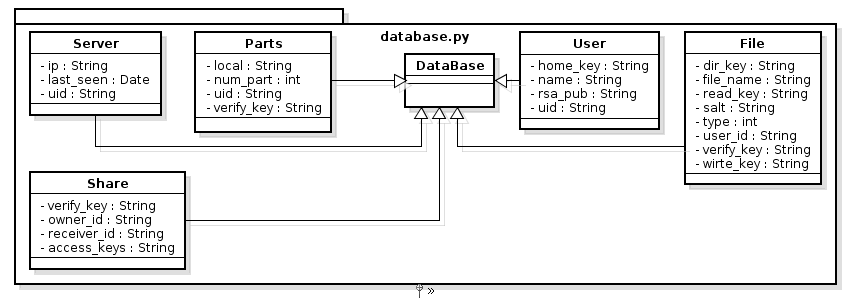
\includegraphics[width=14cm]{shareORM.png}
        \caption{Diagrama de classes mostrando a classe \textit{Share}, responsável por armazenar os metadados sobre o compartilhamento dos arquivos.}
        \label{fig:shareORM}
        \end{figure}
        
        \section{Módulo Cliente para Android}
        
        % - Estudo do Android
        % - Organização do projeto
        % - Modularização
        % - GUI
     
        Um módulo cliente implementado em outra arquitetura é de grande interesse como caso de teste de que as alterações propostas tornam o FlexA capaz de executar em sistemas diferentes e também testar sua nova interface de comunicação, e ainda fornecer ao usuário outra alternativa de uso do sistema.
        
        \subsection{Organização}
        
        Uma das principais contribuições do cliente para Android ao projeto original é a modularização e organização do projeto, separando as funcionalidades e implementação de recursos em pacotes bem definidos com o uso de interfaces de desenvolvimento que forneçam flexibilidade ao projeto.
        
        A modularização do trabalho desenvolvido é mostrada através da arvore de pacotes. Dentro de cada pacote permanecem apenas implementações de tarefas do mesmo tipo. Essa arvore é apresentada na figura \ref{fig:arvorePacotesAndroid}.
        
        \begin{figure}[!ht]
        \centering
        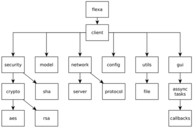
\includegraphics[width=14cm]{pacotesGabriel.png}
        \caption{Hierarquia de pacotes que compõe o módulo Cliente para Android}
        \label{fig:arvorePacotesAndroid}
        \end{figure}
        
        Da forma como o sistema está estruturado, quando no futuro for necessário alterar o módulo cliente ou até mesmo implementar o módulo servidor para Android ou em Java, essa tarefa será bem simples de ser feita pois toda a estrutura do sistema estará pronta, e assim o módulo servidor poderá importar apenas os pacotes que necessita, sem que para isso, seja necessário carregar junto funções e bibliotecas desnecessárias.
        
        \subsection{Modularização e Flexibilidade}
        
        A modularização do projeto ocorre não apenas pelo uso de pacotes e separação do código em classes bem definidas. Para que o projeto possa se manter a longo prazo flexível, são utilizadas diversas interfaces para garantir que caso seja necessário realizar alterações em mecanismos de comunicação e na interface gráfica do usuário ou \textit{Graphical User Interface} (GUI), essas alterações sejam simples de serem implementadas. Os principais pontos são listados a seguir.
        
         \subsubsection{Encapsulamento da complexidade do FlexA}
         
        Embora o XML-RPC forneça um alto grau de encapsulamento da comunicação, ainda é necessário obter uma forma de simplificar o acesso as funções fornecidas pelos servidores XML-RPC e toda a sequência ações que devem ser feitas. Esse encapsulamento é obtido utilizando a classe \textit{Client}, que é mostrada na figura \ref{fig:clientClass}. Dessa forma, caso aconteça qualquer alteração nos protocolos ou nos parâmetros o resto do cliente não precisa ser alterado, ou irá precisar de apenas pequenos ajustes.
        
        \begin{figure}[!ht]
        \centering
        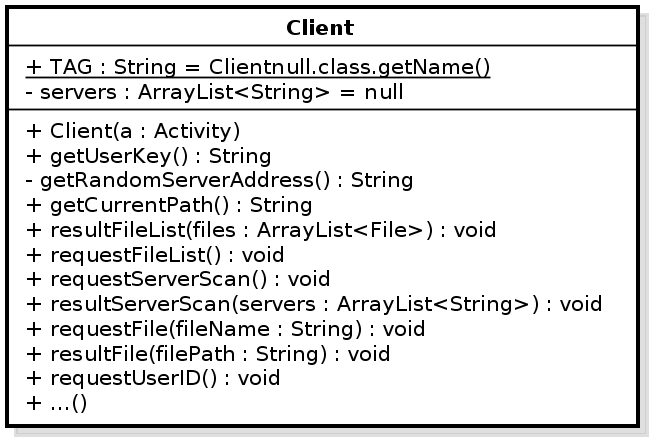
\includegraphics[width=10cm]{classeCliente.png}
        \caption{Classe \textit{Client}, responsável por encapsular servidores e manipulação dos arquivos.}
        \label{fig:clientClass}
        \end{figure}
        
        
         \subsubsection{Encapsulamento da comunicação com os servidores que utilizam XML-RPC}
         
        Ainda sim, para isolar o módulo cliente do cliente XML-RPC utilizado existe a classe \textit{FlexaServer} que é apresentada na figura \ref{fig:flexaServer}. Essa classe é a responsável por se conectar com os servidores RPC e implementar as operações  do lado do cliente mostradas na seção anterior na figura \ref{fig:interfaceComunicacao}.
        
        \begin{figure}[!ht]
        \centering
        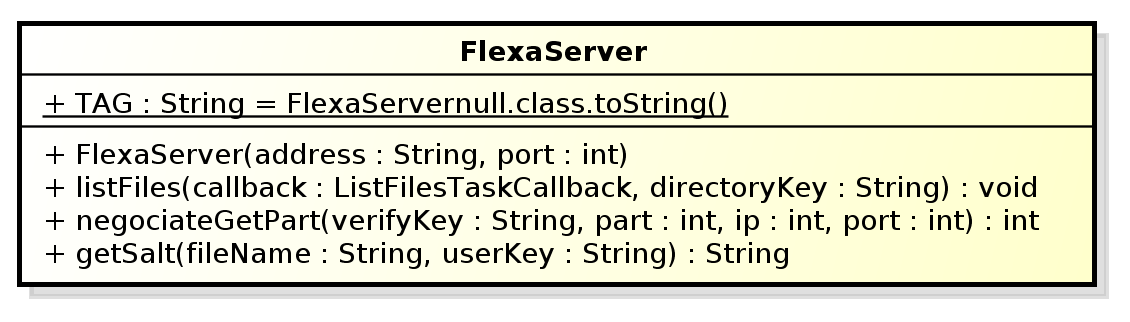
\includegraphics[width=14cm]{flexaServerClass.png}
        \caption{Interface de comunicação com os servidores XML-RPC.}
        \label{fig:flexaServer}
        \end{figure}
        
        
        \subsection{Interface Gráfica do Usuário no Android}
        
        Com as classes \textit{FlexaServer} e \textit{Client}, o resto do módulo cliente fica encapsulado e livre da comunicação com os servidores, devendo assim apenas cuidar da entrada e saída dos dados e da comunicação com o usuário do sistema através de uma interface gráfica. Uma das telas do sistema é exibida na figura \ref{fig:flexaGuiModel}.
        
        \begin{figure}[!ht]
        \centering
        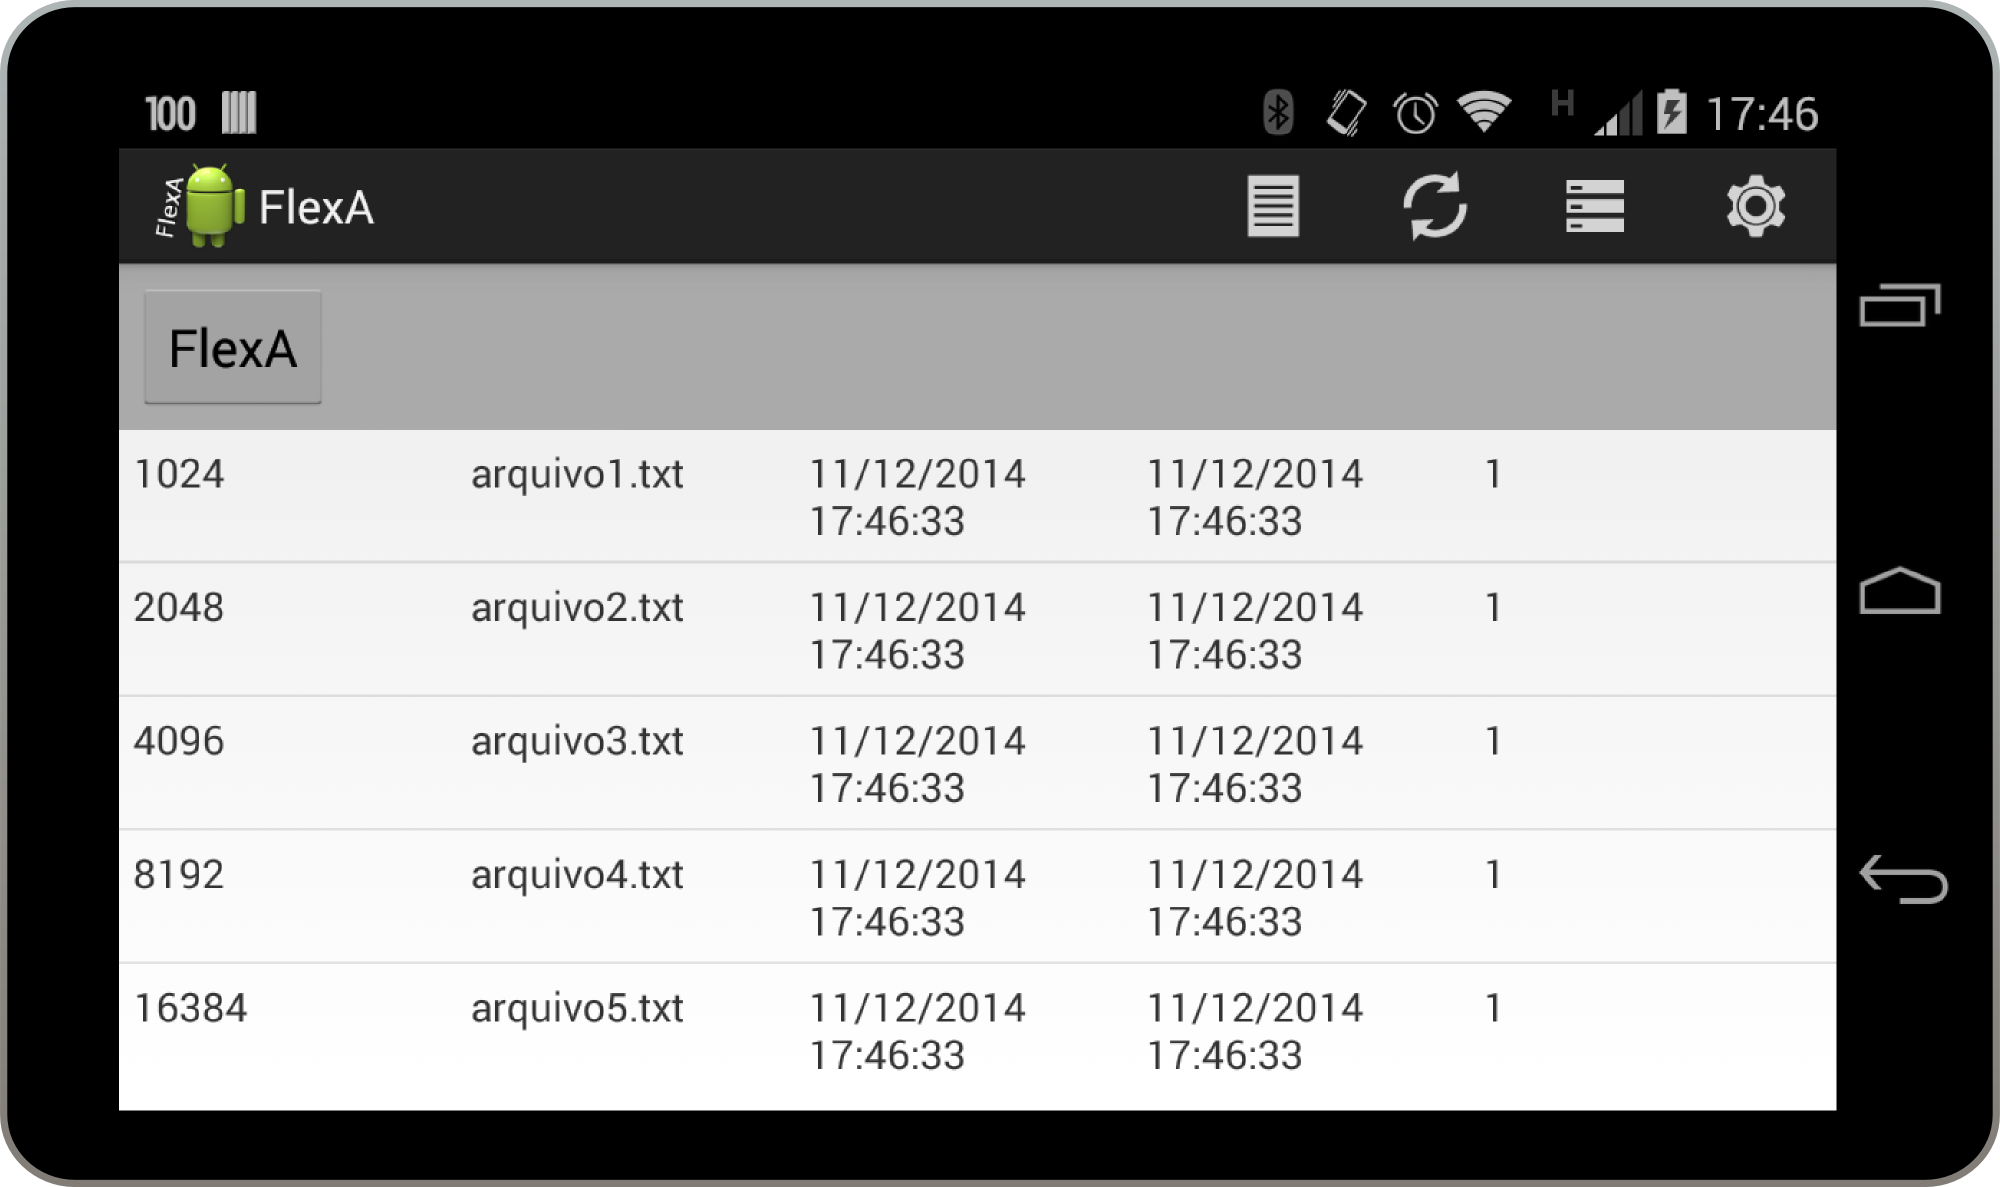
\includegraphics[width=14cm]{flexaGuiModel.png}
        \caption{Exemplo de interface gráfica listando os arquivos do usuário.}
        \label{fig:flexaGuiModel}
        \end{figure}
        
        A utilização de uma GUI para Android, embora seja necessária para a comodidade do usuário final, é bem mais complexa que a implementação para interface de linha de comando ou \textit{Command-line Interface} (CLI) que existe atualmente no cliente em Python. Para obter um resultado satisfatório no uso de uma GUI, é necessário tratar de forma assíncrona e também utilizar \textit{callbacks} nas operações de entrada e saída, de modo a evitar o congelamento do aplicativo ao realizar essas tarefas ~\cite{androidAssyncTask}. Dois exemplos dessas tarefas são mostrados na figura \ref{fig:assyncCallback}.
        
        \begin{figure}[!ht]
        \centering
        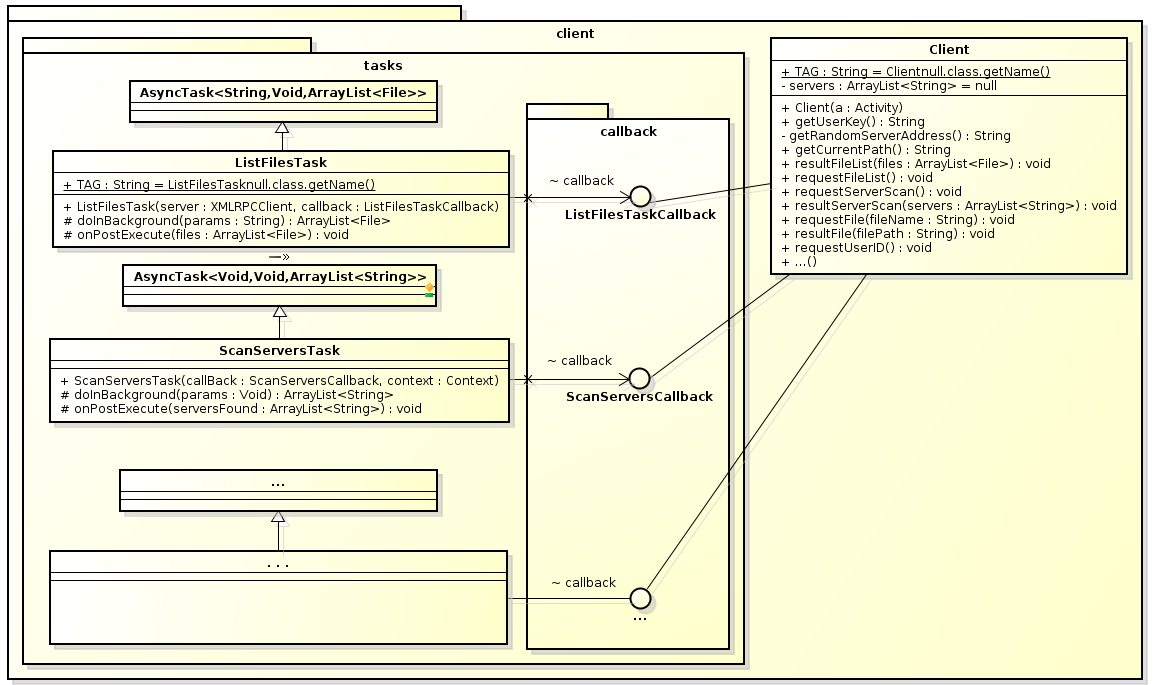
\includegraphics[width=14cm]{assyncCallback.png}
        \caption{Exemplo de duas tarefas assíncronas, uma feita via XML-RPC (\textit{listFiles}) e outra via \textit{socket} (\textit{scanServers}).}
        \label{fig:assyncCallback}
        \end{figure}
        
    Junto com as tarefas assíncronas estão também como exemplo uma parte da classe \textit{Splash} e da interface \textit{FlexaGui} que fazem a conexão com a interface gráfica do cliente que estão destacadas com a cor cinza claro.
    
    Na figura \ref{fig:classesSeg} são apresentados detalhes das classes responsáveis por realizar o processo de segurança com os mecanismos de \textit{hash} e criptografia. Ainda nesta figura estão as classes que fornecem o acesso aos arquivos para a divisão das porções.
    
        \begin{figure}[!ht]
        \centering
        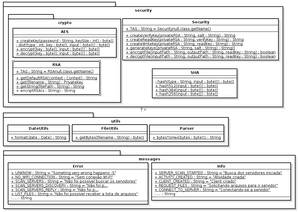
\includegraphics[width=14cm]{classesSegurancaUtils.png}
        \caption{Seções das classes de criptografia e acesso a arquivos.}
        \label{fig:classesSeg}
        \end{figure}
        
    Por fim estão as telas desenvolvidas que fornecem ao usuário acesso as configurações do FlexA, facilitando bastante o processo que anteriormente era feito realizando edições manuais no código fonte. Essas telas são apresentadas na figura \ref{fig:config}.
    
        \begin{figure}[!ht]
        \centering
        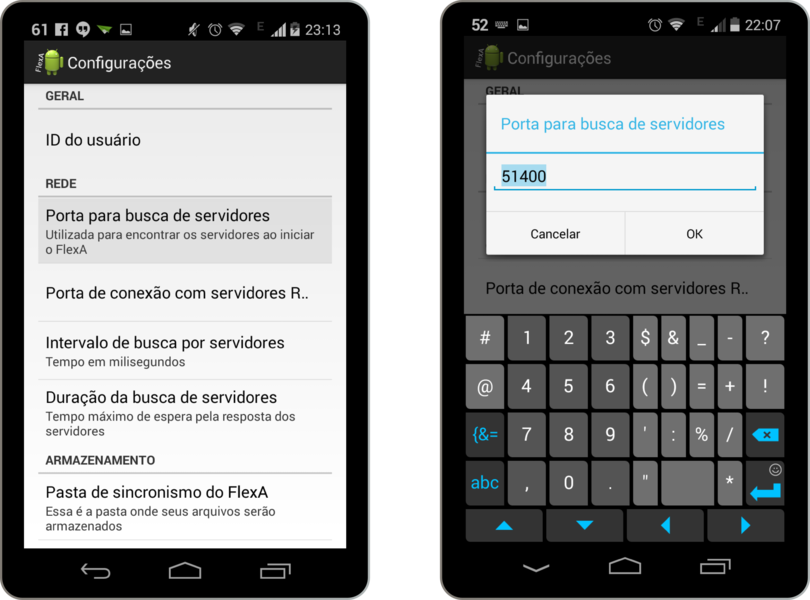
\includegraphics[width=14cm]{androidConfiguracoes.png}
        \caption{Módulo de configurações, fornece uma melhor usabilidade do sistema.}
        \label{fig:config}
        \end{figure}
        
    
    \section{Considerações finais}
    
    Após a descrição do projeto proposto junto com seu desenvolvimento, são apresentados a seguir o cenário e os testes realizados para validar o funcionamento do sistema bem como seu desempenho.